\chapter[High geomagnetic field intensity recorded by anorthosite xenoliths requires a strongly powered late Mesoproterozoic geodynamo][Late Mesoproterozoic geodynamo]{High geomagnetic field intensity recorded by anorthosite xenoliths requires a strongly powered late Mesoproterozoic geodynamo}

\let\thefootnote\relax\footnote{This chapter is published as a peer-reviewed manuscript: Zhang, Y., Swanson-Hysell, N.L., Avery, M.S., Fu, R.R., (2022), High geomagnetic field intensity recorded by anorthosite xenoliths requires a strongly powered late Mesoproterozoic geodynamo. PNAS. doi: \url{https://doi.org/10.1073/pnas.2202875119}.}

\section{Abstract}
Obtaining estimates of Earth's magnetic field strength in deep time is complicated by non-ideal rock magnetic behavior in many igneous rocks. In this study, we target anorthosite xenoliths that cooled and acquired their magnetization within ca. 1092 Ma shallowly emplaced diabase intrusions of the North American Midcontinent Rift. In contrast to the diabase which fails to provide reliable paleointensity estimates, the anorthosite xenoliths are unusually high-fidelity recorders yielding high-quality, single-slope paleointensity results that are consistent at specimen and site levels. An average value of $\sim$83 ZAm$^2$ for the virtual dipole moment from the anorthosite xenoliths, with the highest site-level values up to $\sim$129 ZAm$^2$, are higher than that of the dipole component of Earth's magnetic field today and rival the highest values in the paleointensity database. Such high intensities recorded by the anorthosite xenoliths require the existence of a strongly powered geodynamo at the time. Together with previous paleointensity data from other Midcontinent Rift rocks, these results indicate that a dynamo with strong power sources persisted for more than 14 million years ca. 1.1 Ga. These data are inconsistent with there being a progressive monotonic decay of Earth's dynamo strength through the Proterozoic Eon and could challenge the hypothesis of a young inner core. The multiple observed paleointensity transitions from weak to strong in the Paleozoic and the Proterozoic present challenges in identifying the onset of inner core nucleation based on paleointensity records alone. 


\section{Introduction}
Earth's magnetic field is the result of convective flow of liquid iron-alloy in Earth's outer core. At present day, the geodynamo is collectively powered by heat flow across the core-mantle boundary (CMB) and from the crystallization of the solid inner core from the liquid outer core which provides latent heat and compositional buoyancy due to the exclusion of light elements \citep{Buffett2000a}. However, while paleomagnetic studies have found that a dynamo field has existed since at least 3.4 billion years ago \citep{Selkin2007a, Biggin2011a, Tarduno2014a, Brenner2020a}, Earth's inner core likely crystallized more recently. Estimates of the timing of the initial crystallization of Earth's inner core are interconnected with estimates for the core's thermal conductivity. Higher conductivity values imply faster cooling rates to maintain the geomagnetic field, which in turn imply that the threshold for the crystallization of the inner core happened more recently \citep{Davies2015a}. While some estimated thermal conductivity values are consistent with an inner core age $>$3 Ga \citep{Gubbins2004a, Konopkova2016a}, other estimates have implied higher thermal conductivity values and an age for the inner core that is less than 1.5 Ga \citep{Pozzo2012a, Koker2012a, Gomi2013a, Zhang2020b, Frost2022a}, with some suggesting even younger ages ($<$700 Ma; \cite{Labrosse2015a, Ohta2016a, Pozzo2022a}). The possibility of late inner core nucleation has motivated proposals of novel power sources to sustain the geomagnetic field through early Earth history including precipitation of light-element minerals such as MgO \citep{Badro2016a, ORourke2016a, ORourke2016b} and SiO$_2$ \citep{Mittal2020a} at the core-mantle boundary. Given that estimates for the core's thermal conductivity continue to be debated, it is crucial to use observational records as an independent constraint on the thermal evolution of Earth's core and mantle.

Paleomagnetic records from ancient rocks are one of the few types of observational data that have the potential to provide constraints on the thermal evolution of Earth’s core. Evidence for a persistent magnetic field through the Proterozoic, for example, likely necessitates the existence of plate tectonics that sustained core-mantle boundary heat flow \citep{Swanson-Hysell2021c}. However, strikingly low estimates of geomagnetic field strengths have been obtained ca. 565 Ma during the Ediacaran Period \citep{Bono2019a, Shcherbakova2019a,Thallner2021b} and ca. 370 Ma during the Devonian Period \citep{Shcherbakova2017a, Shcherbakova2021a, Hawkins2021a}, potentially indicating unusual periods of core dynamo activity at those times. The Ediacaran data have been interpreted to indicate that there was a progressively decaying field up to that time that was soon followed by initial crystallization of the inner core \citep{Bono2019a}. Sparse paleointensity data in the Proterozoic Era (2500 to 539 Ma) and the reality of high variability in Phanerozoic Era records (539 to 0 Ma) necessitate additional data to evaluate interpreted trends. 

\begin{figure}[h!]
\centering
\noindent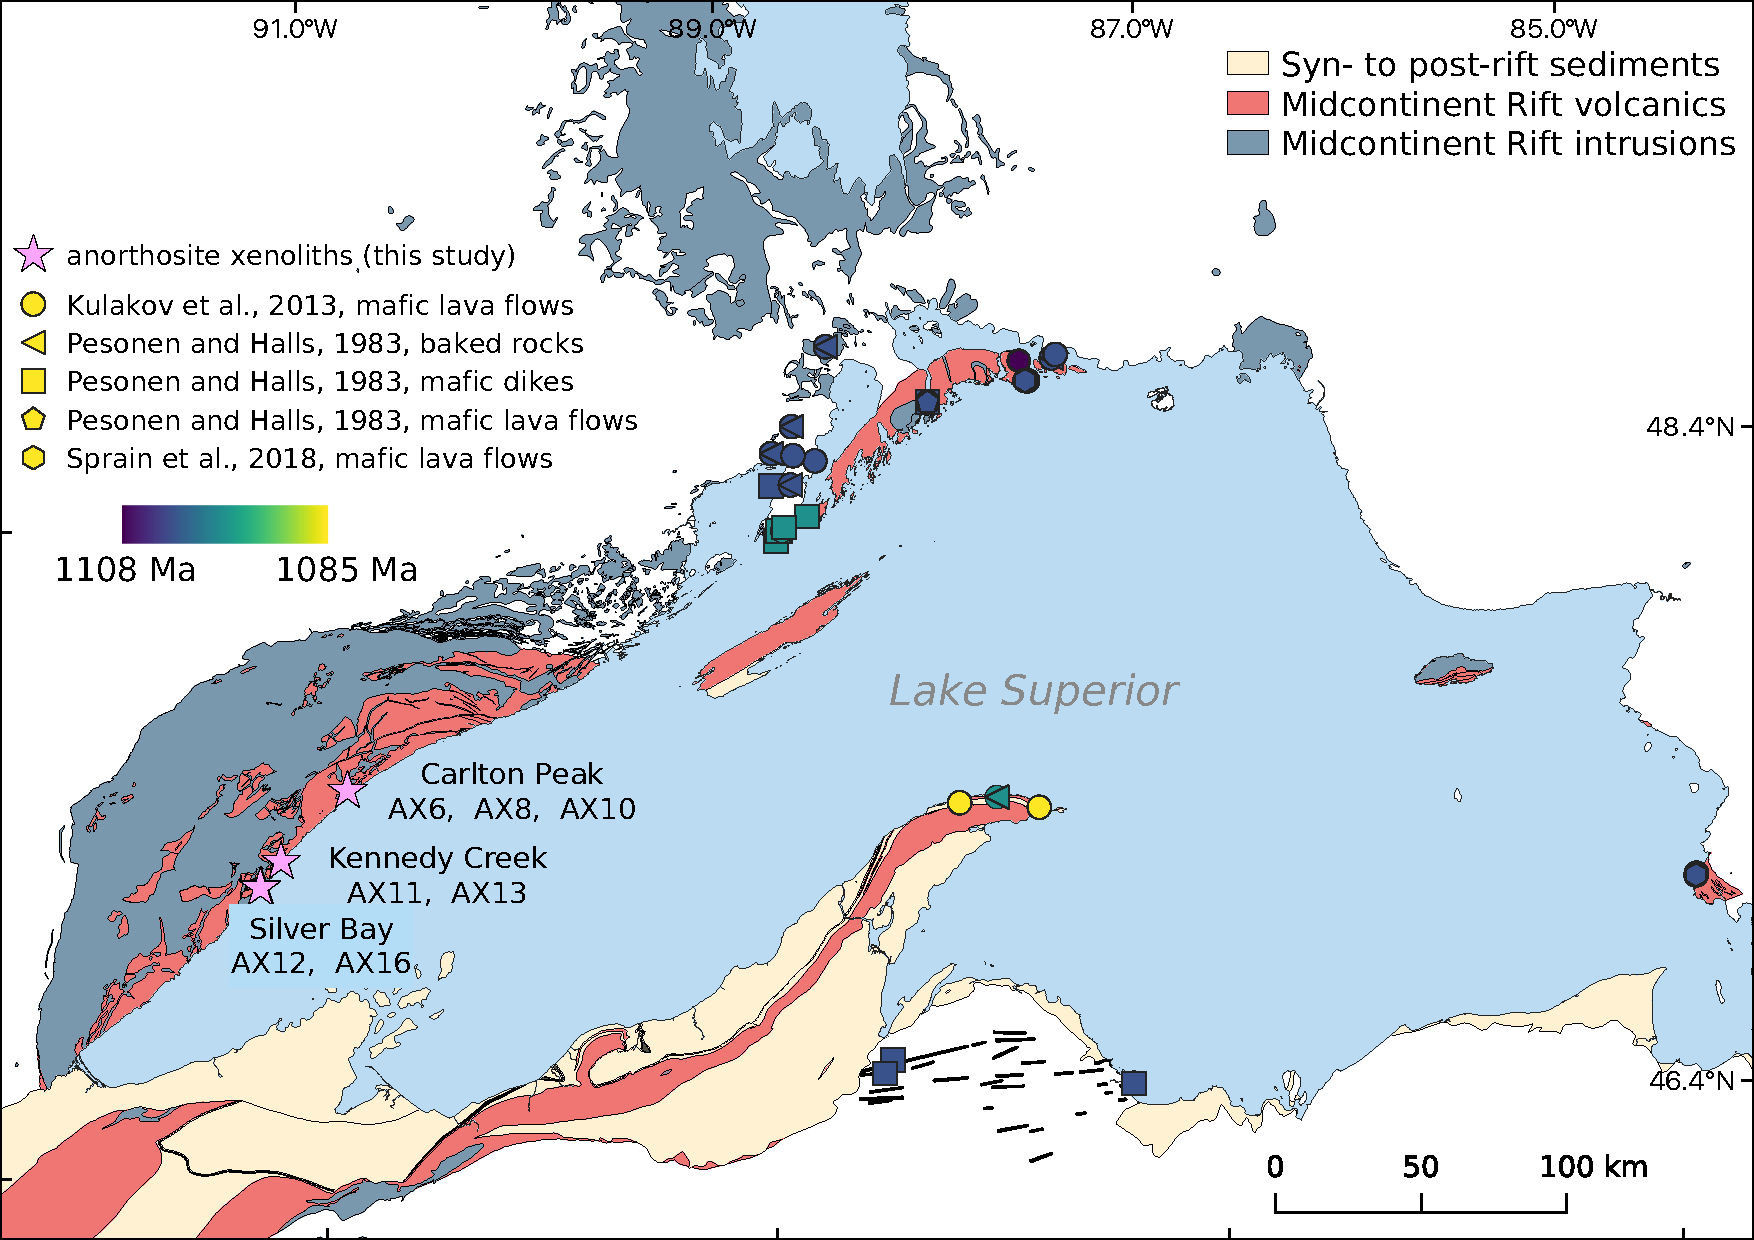
\includegraphics[width=0.9\textwidth]{figure/Zhang2022/Geologic_map.pdf}
\caption{\footnotesize{Simplified geologic map of the Lake Superior region showing the distribution of rocks associated with the late Mesoproterozoic Midcontinent Rift. Purple stars mark sites with paleointensity results that passed the selection criteria from this study. Paleomagnetic sites from \citealp{Pesonen1983a} are categorized by lithology. All sites from refs. \citealp{Pesonen1983a, Kulakov2013a, Sprain2018a} are color-coded by their ages.}}
\label{fig:Chap_PINT_Geologic_map}
\end{figure}

Determinations of the absolute value of ancient geomagnetic field strength rely on igneous rocks that acquire thermal remanent magnetizations as they cool. These magnetizations need to be unmodified by subsequent heating or chemical alteration in order to maintain the record of the ancient geomagnetic field from the time of cooling. Intracontinental magmatic events are an important target for determination of ancient paleointensity as they can be well-preserved within continental interiors. This interior position results in them typically being distant from tectonic events along continental margins that can drive alteration through heat and fluid flow. However, intraplate magmatism associated with large igneous provinces is typically of geologically short duration with the bulk of magmatic products emplaced within 1 Myr or less \citep{Kasbohm2021a}. The Midcontinent Rift (Fig. \ref{fig:Chap_PINT_Geologic_map}) is an exception as it is a large igneous province where magmatism lasted $\sim$25 Myr from \textit{ca.} 1109 Ma to 1084 Ma during which there were pulsed intervals of more rapid magmatic activity \citep{Swanson-Hysell2021a}. Additionally, extension ceased in the Midcontinent Rift prior to lithospheric separation, preserving volcanic, intrusive, and sedimentary rocks of the rift within the continental interior far from the continental margin and subsequent orogenesis. As a result, rocks of the rift have unusually simple paleomagnetic behavior for their greater than one billion-year-old age and paleomagnetic data from rift rocks form a central record of Mesoproterozoic paleogeography \citep{Swanson-Hysell2021c}. The duration of magmatic activity within the Midcontinent Rift is longer than the entire 20.4 Myr long Neogene Period such that it provides an extended well-preserved window into the intensity of Earth's magnetic field in the late Mesoproterozoic. 

Despite the excellent preservation of the rocks, non-ideal paleointensity behaviors have posed challenges for the interpretation of many previous paleointensity results from the Midcontinent Rift \citep{Pesonen1983a, Kulakov2013a, Sprain2018a}. The most trusted type of paleointensity estimate is that obtained through experiments in which the primary natural remanent magnetization (NRM) is progressively replaced by a laboratory magnetization that is imparted in a known field with internal consistency checks (such as in IZZI-style Thellier experiments;  \citealp{Yu2004a}). In such Thellier paleointensity experiments, one typical departure from ideal behavior due to the presence of nonuniformly magnetized grains (with either multidomain \citep{Dunlop2001a} or vortex states \citep{Tauxe2020a}) is sagging or double-slopes as visualized in Arai plots that show thermal remanent magnetization (TRM) acquired versus NRM lost. For such data, distinct paleointensity estimates may be calculated depending on the interpreter's choice of slope. Typically, such non-ideal behavior would result in a higher paleointensity estimate from the steeper-sloped low-temperature portion of the experiment and a lower paleointensity estimate from the high-temperature portion. For example, in data from the Midcontinent Rift, \citealp{Pesonen1983a} used the low-temperature slope as the best representation of the past magnetic field strength (likely overestimating the field strength) whereas \citealp{Kulakov2013a} used the high-temperature slope (likely underestimating the field strength). Such non-ideal results were rejected by \citealp{Sprain2018a} who applied stricter paleointensity selection criteria, but as a result had few accepted sites.

In this study, we target the high-purity anorthosite xenoliths of the Beaver River diabase in the Midcontinent Rift. While magmatic activity within the Midcontinent Rift was protracted, there were intervals of particularly rapid volcanism and voluminous emplacement of intrusions \citep{Swanson-Hysell2021a}. The ca. 1092 Ma Beaver Bay Complex in northern Minnesota punctuates one such period of magmatism during the main stage of Midcontinent Rift activity. The magma that formed the 1091.7$\pm$0.2 Ma Beaver River diabase dikes and sills of the Beaver Bay Complex transported numerous anorthosite xenoliths that have short-axis diameters up to 180 meters via wide conduits \citep{Boerboom2004a, Boerboom2006b}. These anorthosite xenoliths are plagioclase cumulates that formed comagmatically with the host diabase in the lower crust---an interpretation confirmed by U-Pb zircon geochronology \citep{Zhang2021b}. They are attractive targets for paleomagnetic study as plagioclase crystals can protect magnetic inclusions from alteration. In addition, the alteration of the plagioclase crystals does not readily result in the formation of secondary iron oxides in contrast with Fe-silicate minerals such as olivine and pyroxene. The anorthosite xenoliths targeted in this study were brought to the near surface in magma that formed hypabyssal (shallowly emplaced) intrusions of the Beaver River diabase \citep{Zhang2021b}. They would have been heated to tholeiitic magma temperature ($\sim$1100\textdegree C) which is below the melting point of the xenolith plagioclase (70$\%$ anorthite), but well above the Curie temperature of magnetite \citep{Zhang2021b}. Fe-Ti oxides within the plagioclase likely exsolved above magnetite Curie temperature \citep{Bian2021a} and subsequently cooled and acquired thermal remanent magnetizations in conjunction with the host diabase at a paleolatitude of 22 $\pm$ 2\textdegree$\;$(calculated from the paleomagnetic pole of the coeval Portage Lake Volcanics; \citealp{Swanson-Hysell2019a}). Paleointensity experiments on the anorthosite xenoliths have a high success rate, yielding consistent specimen- and site-level paleointensity results. The anorthosite xenoliths show low anisotropy of thermal remanent magnetization acquisition and can acquire TRM linearly within the range of relevant field strengths. Magnetic imaging shows that the anorthosite specimens have dominant magnetic carriers within and interstitial to plagioclase crystals without strong preferred orientations. Thermal modeling results and paleomagnetic directional data show that the anorthosite xenoliths acquired thermal remanent magnetizations while cooling with the Beaver River diabase \citep{Zhang2021b}. Step-wise thermal demagnetization data show the anorthosite xenoliths to have dominantly single-component magnetizations that often unblock sharply within temperature ranges between 500\textdegree C and 580\textdegree C, consistent with remanence being held by low-titanium titanomagnetite \citep{Zhang2021b}. 

\begin{SCfigure*}
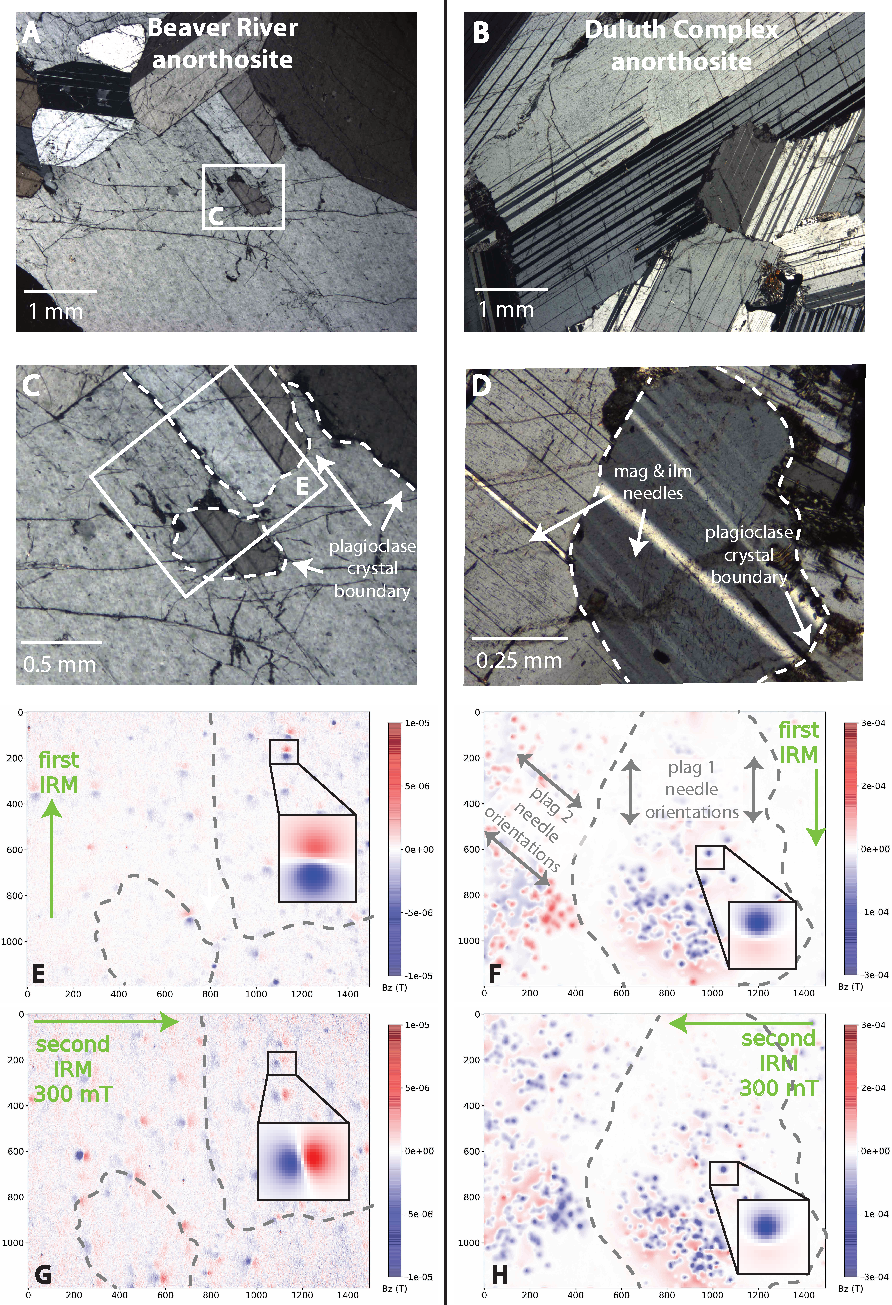
\includegraphics[width=0.6\textwidth]{figure/Zhang2022/Petro_QDM_full.pdf}
\caption{\tiny Thin section petrographic images (A,B,C,D) and magnetic maps (E,F,G,H) of an anorthosite sample from the Beaver River anorthosite xenolith in the Silver Bay region from which paleomagnetic site AX16 and geochronology sample MS99033 were collected (left column;  \citealp{Zhang2021b}) and from a distinct anorthosite within the Duluth Complex Anorthositic Series (right column). The Duluth Complex anorthosites were not targeted for paleointensity experiments in this study given complexities associated with more pronounced fabrics. Cross-polarized petrographic images of the Beaver River anorthosite (A,C) reveal plagioclase with a granoblastic texture of crystals that are largely free of large opaque inclusions. In contrast, plagioclase crystals in the Duluth Complex anorthosite have euhedral, interlocking crystals with an igneous foliation (B) and the plagioclase crystals contain abundant Fe-Ti oxide needles that have preferred orientations that are often parallel with the [001] axis of the plagioclase. Maps of the vertical component of magnetic field (B$_z$) developed with a quantum diamond microscope (QDM) show relatively weak magnetic sources within plagioclase crystals in the Beaver River anorthosite (in E) relative to the strongly magnetic large oxide needles within Duluth Complex plagioclase (in F). The B$_z$ color scale is an order of magnitude greater in the Duluth Complex anorthosite maps (F, H) than the maps for the Beaver River anorthosite (E, G). Panels (E) to (G) and (F) to (H) show experiments performed on both samples where we apply a first field along the y-axis of the field of view and then apply a second field of 300 mT orthogonal to the first field direction. The remanent magnetizations acquired by both anorthosites were mapped after the application of each field. The magnetic images show that remanent magnetizations of Beaver River anorthosite (i.e. the individual dipoles visible with paired red +B$_z$ and blue -B$_z$ lobes) align well with the first applied field direction (E) and then rotated to align with the second applied field direction indicating minimal anisotropic behavior (G). In contrast, the remanent magnetizations carried by the magnetic needles in plagioclase 1 of the Duluth anorthosite xenolith align well with the first applied field but those in plagioclase 2 acquired an oblique remanence direction with respect to the field direction (F). After the application of an orthogonal 300 mT external field, magnetization of those needles in plagioclase 1 did not change direction due to strong shape anisotropy whereas the magnetization of needles in plagioclase 2 flipped, but with the acquired remanence remaining oblique to the field direction (H). Insets in (E) to (H) show example dipole directions (fit using the algorithm of \citep{Lima2016a}) in response to the application of orthogonal IRMs. The directional changes of the Beaver River anorthosite xenolith sources indicate a lower magnetic anisotropy compared to the relative lack of change for the Duluth Complex anorthosite xenolith sources. The unit of the axes in the QDM maps are in $\mu$m.}
\label{fig:Petro_QDM}
\end{SCfigure*}

\section{Results and Interpretations}

\subsection*{Petrography and magnetic imaging of anorthosite xenoliths}

The dominantly monomineralic anorthosite xenoliths within the Beaver River diabase often have granoblastic texture characterized by equigranular crystals with weakly developed petrofabrics (Fig. \ref{fig:Petro_QDM}A). Plagioclase crystals within coarse-grained intrusions often contain abundant elongate Fe-Ti oxide inclusions that are visible with optical microscopy \citep{Feinberg2006a, Wenk2011a, Ageeva2016a}. The Beaver River anorthosite xenoliths lack such large (10s of $\mu$m) oxide inclusions such that the oxides are not visible within the plagioclase crystals using optical microscopy (Fig. \ref{fig:Petro_QDM}C). Magnetic imaging using a quantum diamond microscope (QDM), however, shows that there are magnetic remanence carriers within the plagioclase crystals (Fig. \ref{fig:Petro_QDM}E, G). The sources of these magnetic remanence carriers are likely to be Fe-Ti oxides that exsolved within plagioclase crystals above the Curie temperature of magnetite \citep{Zhang2021b, Bian2021a}. To highlight these distinctive aspects of the Beaver River anorthosite xenoliths, we present petrographic and magnetic imaging data from the Beaver River anorthosite as well as an anorthosite sample from the Duluth Complex Anorthositic Series---an older intrusive complex within the Midcontinent Rift that was not targeted for paleointensity experiments in this study (Fig. \ref{fig:Petro_QDM}). In contrast to the Beaver River anorthosite, the plagioclase crystals of this Duluth Complex anorthosite sample has a pronounced igneous foliation (Fig. \ref{fig:Petro_QDM}B). In addition, there are abundant Fe-Ti oxide needles within the Duluth Complex plagioclase grains that are typically aligned with the [001] axes of the crystals (Fig. \ref{fig:Petro_QDM}D). Magnetic imaging confirms that these needles have magnetic moments oriented along their long axes (Fig. \ref{fig:Petro_QDM}F, H). As a result of this shape anisotropy, remanent magnetizations are acquired at angles highly oblique to applied fields (Fig. \ref{fig:Petro_QDM}F). In an experiment where a second orthogonal field was applied, the first isothermal remanent magnetizations (IRM) of a set of magnetite needles within a plagioclase grain either fail to rotate or flip by 180\textdegree. When they flip, they remain in a direction that is oblique to the applied field direction dictated by shape anisotropy (Fig. \ref{fig:Petro_QDM}F, H). These experiments enable novel visualization of the grain-scale magnetic anisotropy of elongated exsolved (titano)magnetite inclusions within plagioclase grains that leads to magnetic anisotropy observed at the bulk sample scale \citep{Selkin2000a, Feinberg2006a}. In contrast, the remanent magnetizations of the ferromagnetic grains imaged in the Beaver River anorthosite xenoliths, targeted for paleointensity in this study, align with the applied field directions indicating minimal remanence anisotropy  (Fig. \ref{fig:Petro_QDM}E, G). The relative lack of petrofabrics and minimal grain-scale magnetic anisotropy make the Beaver River anorthosite xenoliths a particularly compelling target for paleointensity experiments.

\subsection*{Paleointensity}

Following IZZI-style paleointensity experiments \citep{Yu2004a}, 40 from a total of 86 anorthosite specimens and 0 out of a total of 69 diabase specimens passed our paleointensity result selection criteria (see Materials and Methods section). Seven anorthosite sites and no diabase sites have specimen results that pass these selection criteria. Example NRM/TRM (Arai) plots are shown in Figure \ref{fig:IZZI_examples}. Summary specimen absolute paleointensity estimates and site-level mean paleointensity values are plotted in Figure \ref{fig:PINT_cooling_corrected} (and provided in Table S1) where each site represents an individual anorthosite xenolith. The paleointensity quality index (Q$_{PI}$; \citealp{Biggin2014a}) for the anorthosite xenolith sites are all 5 or 6 (Table S2). The cooling rate-corrected absolute paleointensity estimates from the anorthosite xenoliths have a mean of 38.86 $\pm$ 12.10 $\mu$T. The site-mean virtual dipole moment is $\sim$83 ZAm$^2$ ($10^{21} Am^2$) ca. 1092 Ma. All measurement-level paleointensity experiment data are available within the MagIC database (\url{https://doi.org/10.7288/V4/MAGIC/19462}). 

\begin{figure*}
\noindent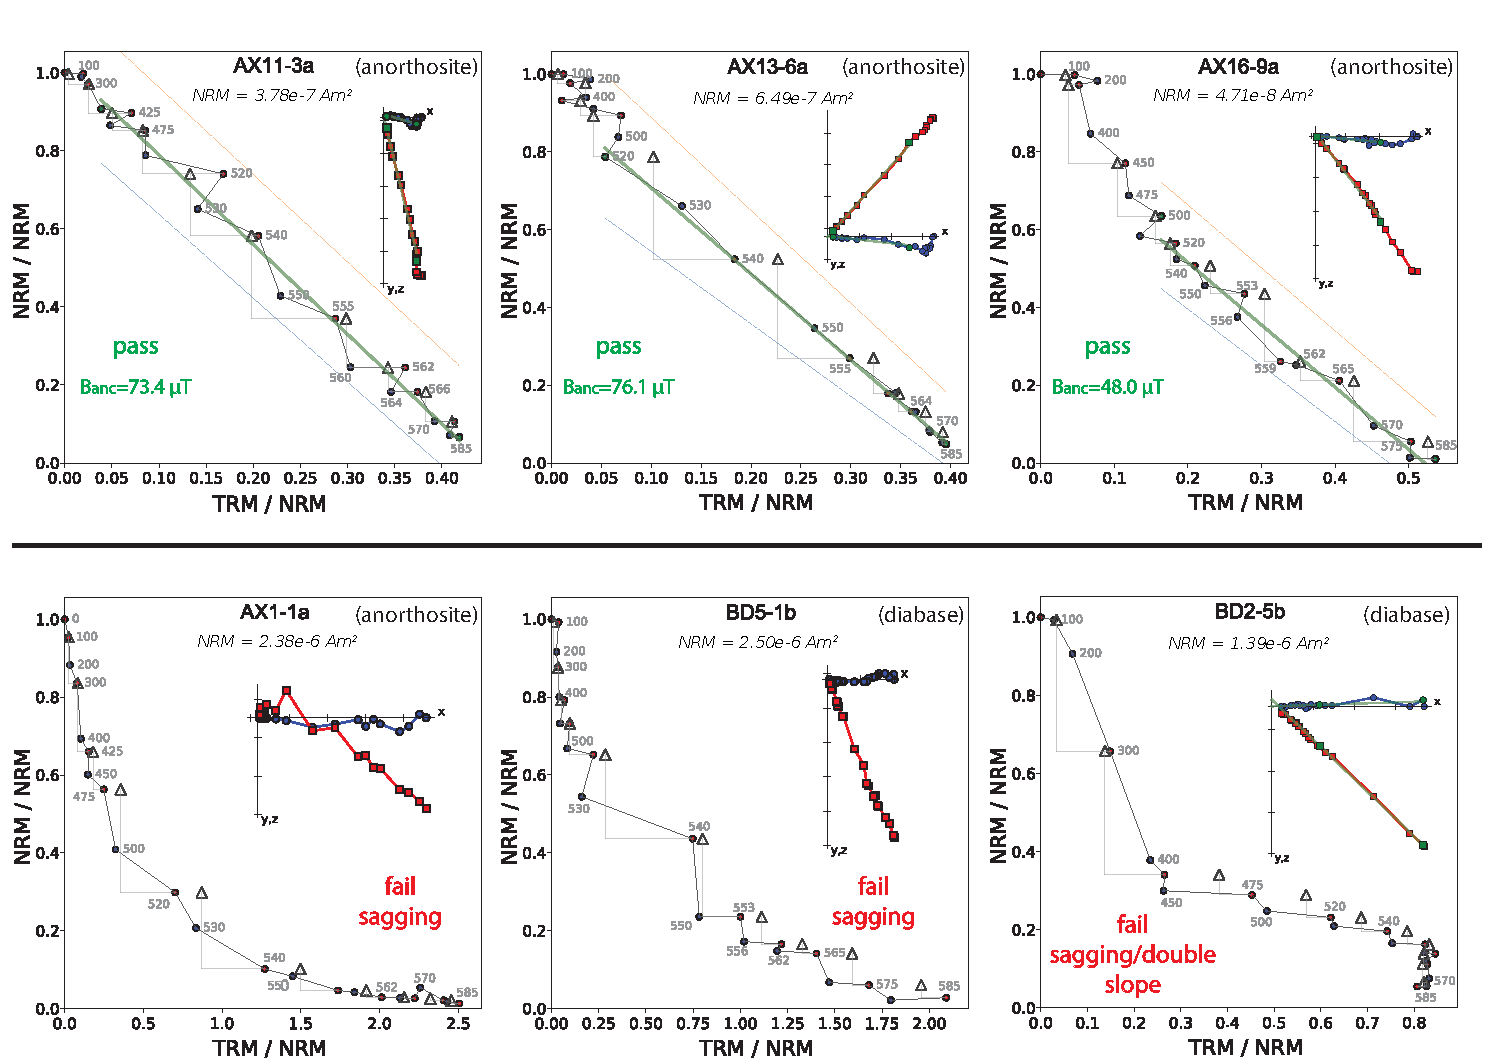
\includegraphics[width=\textwidth]{figure/Zhang2022/IZZI_examples.pdf}
\centering
\caption{\footnotesize{Example results of paleointensity experiments are displayed on Arai plots and zero-field heating results are shown as inset orthogonal plots (Zijderveld plots) for anorthosite and diabase specimens. Green squares and lines in Arai plots and green squares in orthogonal plots show the range of data points used for fitting. Red (blue) circles indicate zero-field/in-field (in-field/zero-field) steps `ZI’'(`IZ'). Triangles mark partial thermal remanent magnetization (pTRM) checks. Blue and red squares in the Zijderveld plots are X–Y and X–Z projections, respectively, of the NRMs in specimen coordinates. Dashed red and blue lines show bounding regions associated with the \textit{SCAT} statistic \citep{Shaar2013a}. Plots on the top row show successful specimen paleointensity results with straight, single-slope behaviors that pass our selection criteria. The green lines represent fits for the dominant single-slope component that passes the acceptance criteria and gives an estimate of the ancient field strength (B$_{anc}$). The plots for anorthosite specimens AX1-1a and diabase BD5-1b on the bottom row show non-ideal sagging behaviour that fails our acceptance criteria. Specimen BD2-5a is an example where the data appear linear with distinct slopes in the low and high temperature ranges such that it could pass less restrictive selection criteria, particularly if a narrower temperature range was used for the experiment. Data analysis and visualization was conducted using PmagPy \citep{Tauxe2016a}.}}
\label{fig:IZZI_examples}
\end{figure*}

Typical paleointensity experimental data of the anorthosite specimens have straight, single-slope NRM/TRM plots and the accepted fractions of temperature steps span over the origin-trending, primary remanence components (Fig. \ref{fig:IZZI_examples}). We accept specimen- and site-level absolute paleointensity results from those anorthosite xenoliths that pass the selection criteria. Other anorthosite xenoliths and diabase specimens failed the selection criteria largely because of double-slope or sagging behavior (fail FRAC selection; see Materials and Methods section), poor pTRM checks, and zigzagging behaviors occasionally superimposed on top of sagging behavior (fail SCAT, DANG selection; see Materials and Methods section; Fig. \ref{fig:IZZI_examples}). A 20 mT alternating field treatment after in-field heating steps was applied to some specimens, but this treatment did not result in significant changes in the experimental results for the anorthosite xenolith or diabase specimens (Fig. \ref{fig:PINT_cooling_corrected}). 

\begin{figure*}[h!]
\noindent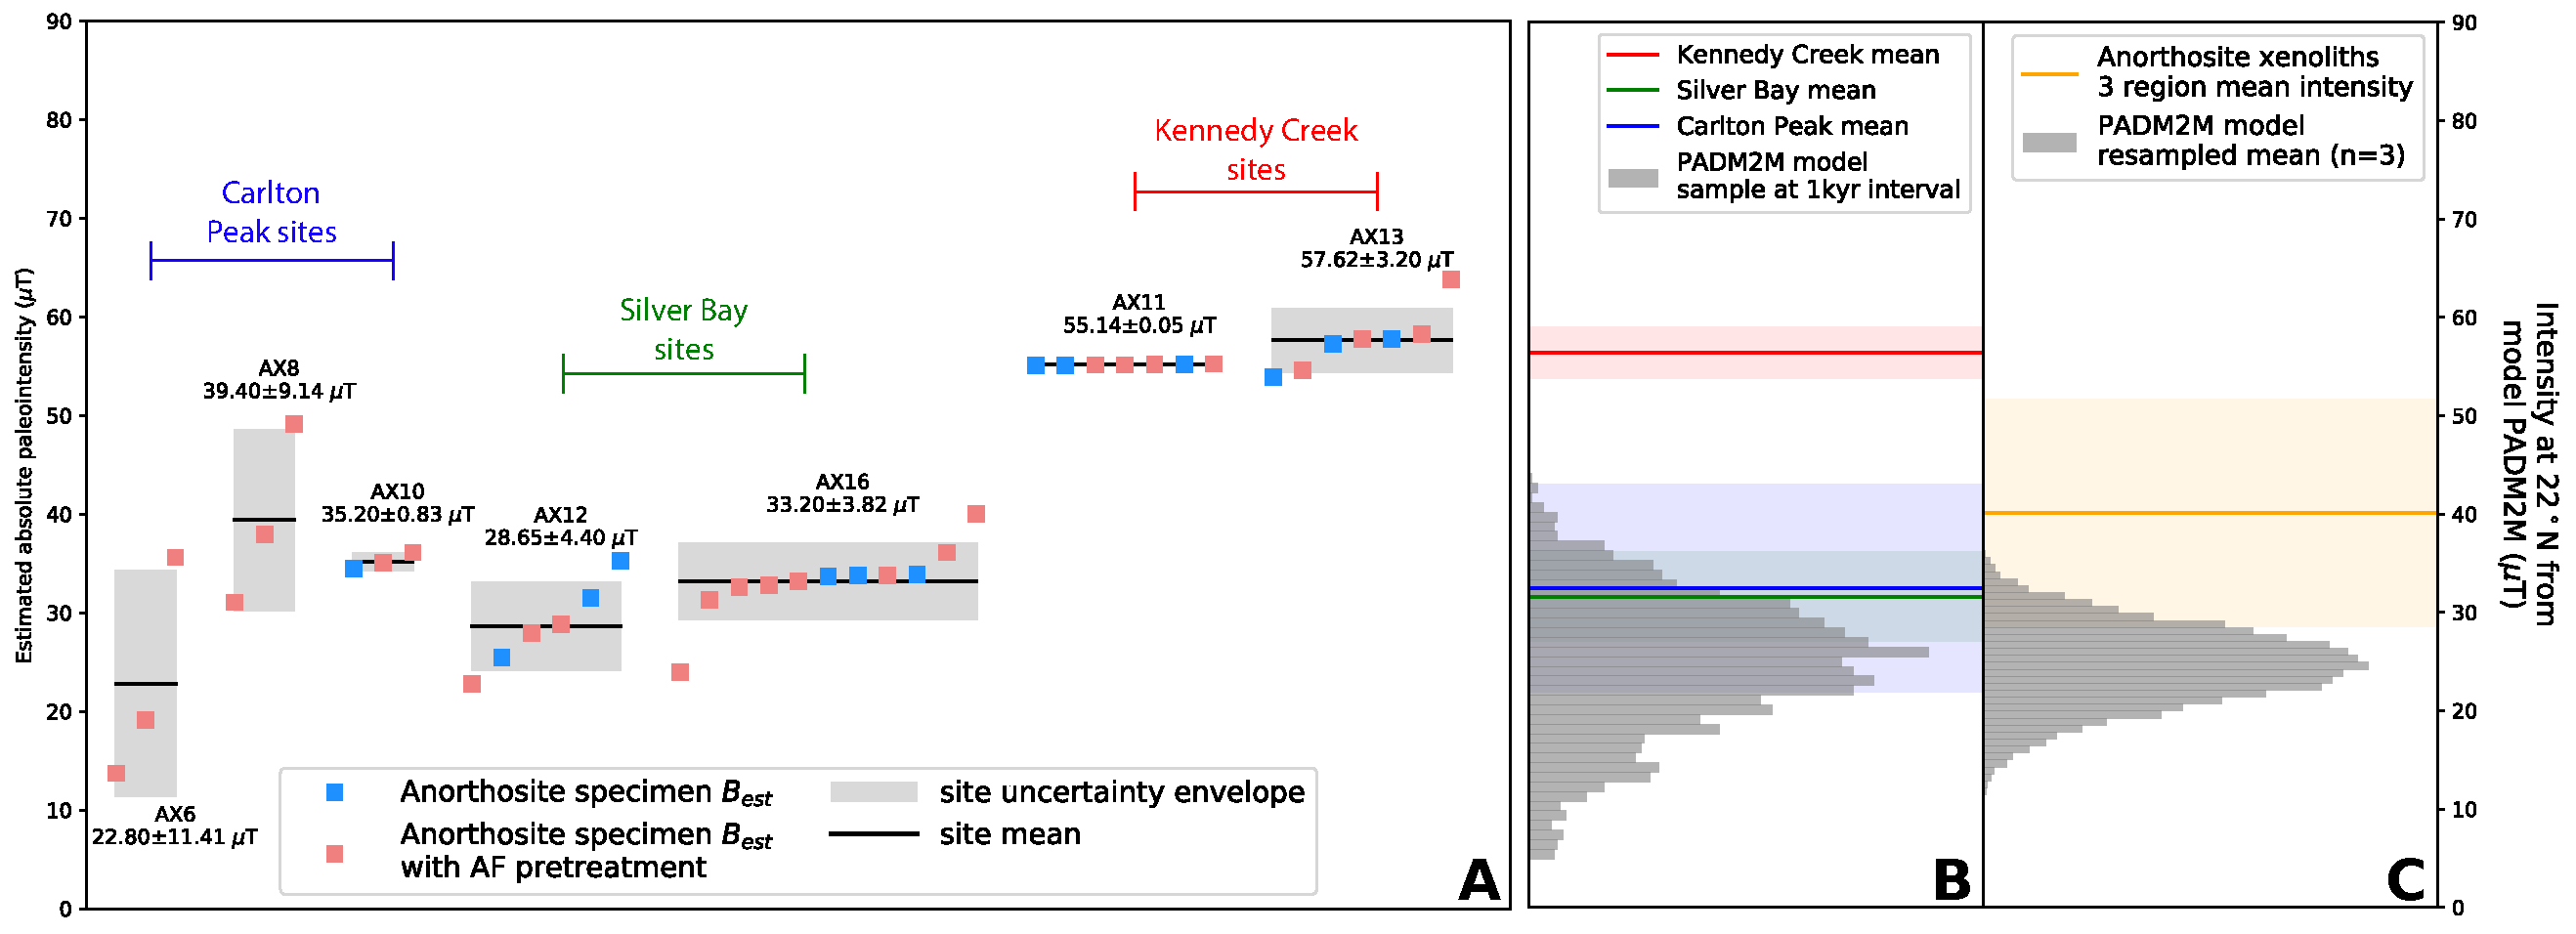
\includegraphics[width=\textwidth]{figure/Zhang2022/Paleointensity_plot_cooling_corrected.pdf}
\centering
\caption{\footnotesize{(A) Summary plot of individual specimen absolute paleointensity results (square symbols) and their averages and standard deviations at site level (black bars with grey one standard deviation uncertainty envelopes) where each `AX' site is an individual anorthosite xenolith within the Beaver River diabase. All results are corrected for cooling rate bias with a factor of 0.75. The sites with successful experiments come from 3 regions (Carlton Peak, Silver Bay, Kennedy Creek) which would have cooled at distinct times yielding similar estimates within each region with differences between regions. (B) Regional means calculated from the specimen-level data are compared to the distribution of intensities calculated from a paleomagnetic axial dipole moment model for the past 2 million years (PADM2M; \citealp{Ziegler2011a}) at the latitude corresponding to the paleolatitude of study region (22\textdegree N). (C) The mean of the 3 regional means is compared to means calculated from 3 random values drawn from the PADM2M model \citep{Ziegler2011a}. The distribution represents a total of 10,000 iterations of taking 3 random draws and calculating the mean. These comparisons highlight that these anorthosites' paleointensity values are strong in relation to the geomagnetic field over the past 2 million years. All shaded regions in (B) and (C) represent one standard deviation uncertainties.}}
\label{fig:PINT_cooling_corrected}
\end{figure*}

In addition to estimating paleointensity values by introducing a set of selection criteria to filter our experiment results, we applied an independent statistical method from \citealp{Cych2021a} to all experimental data regardless of their NRM/TRM plot statistics to make a bias-corrected estimation of paleointensity (BiCEP). This Bayesian probabilistic method is based on the assumption that paleointensity estimates from specimens that come from a same cooling unit are distributed around a true paleointensity value with the various deflections being expressed as the curvature parameter of the NRM/TRM plot \citep{Paterson2011a}. The posterior paleointensity distributions from these sites with high-quality specimen-level data are in agreement with the site-level averages developed using the selection criteria approach (Fig. \ref{fig:PINT_cooling_corrected}; Fig. S1). Overall, the high-quality results from the anorthosite xenoliths of the Beaver River diabase indicate that the anorthosite xenoliths record a high geomagnetic field ca. 1092 Ma. 

\subsection*{Rock magnetism}
\subsubsection*{Coercivity}
Additional rock magnetic data indicate that those anorthosite specimens which pass the paleointensity selection criteria contain dominant magnetic remanence carriers with magnetic properties similar to stoichiometric, non-interacting, single domain magnetite, whereas anorthosite samples that failed the paleointensity result selection along with all diabase samples have more pronounced populations of non-ideal carriers. Magnetic property measurement system (MPMS) data show that both the diabase and anorthosite contain (titano)magnetite as evidenced by the presence of the Verwey transition (Fig. S2;  \citealp{Verwey1939a, Feinberg2015a}). Anorthosite specimens from sites that yield successful paleointensity results have Verwey transition temperatures near 120 K as expected for stochiometric magnetite with minimal Ti contents \citep{Ozdemir1993a}. However, diabase and anorthosite specimens that did not pass our paleointensity selection typically have Verwey transitions that are suppressed toward lower temperatures (Fig. S2), indicating that their magnetic grains either have relatively higher Ti content or have been partially oxidized \citep{Ozdemir1993a}. Another difference is that samples which pass paleointensity selection have distinctly higher average median destructive field values than other anorthosite and diabase specimens (Fig. \ref{fig:coercivity}). Single-component fits for coercivity spectra \citep{Maxbauer2016a} show that anorthosites having successful paleointensity results can contain magnetic grain populations that have higher coercivities. For these successful samples, median destructive (MDF) field values associated with back-field demagnetization experiments range from 44 to 144 mT with a median of 53 mT (Fig. \ref{fig:coercivity}). In contrast, other anorthosite and diabase specimens tend to have lower peak coercivities (MDF range of 18-35 mT with a median of 22 mT; Fig. \ref{fig:coercivity}). This result is consistent with an interpretation that magnetic grain populations with more multidomain-like behavior are responsible for the non-ideal paleointensity behaviors during experiments of such specimens \citep{Xu2004a}.

\begin{figure}
\noindent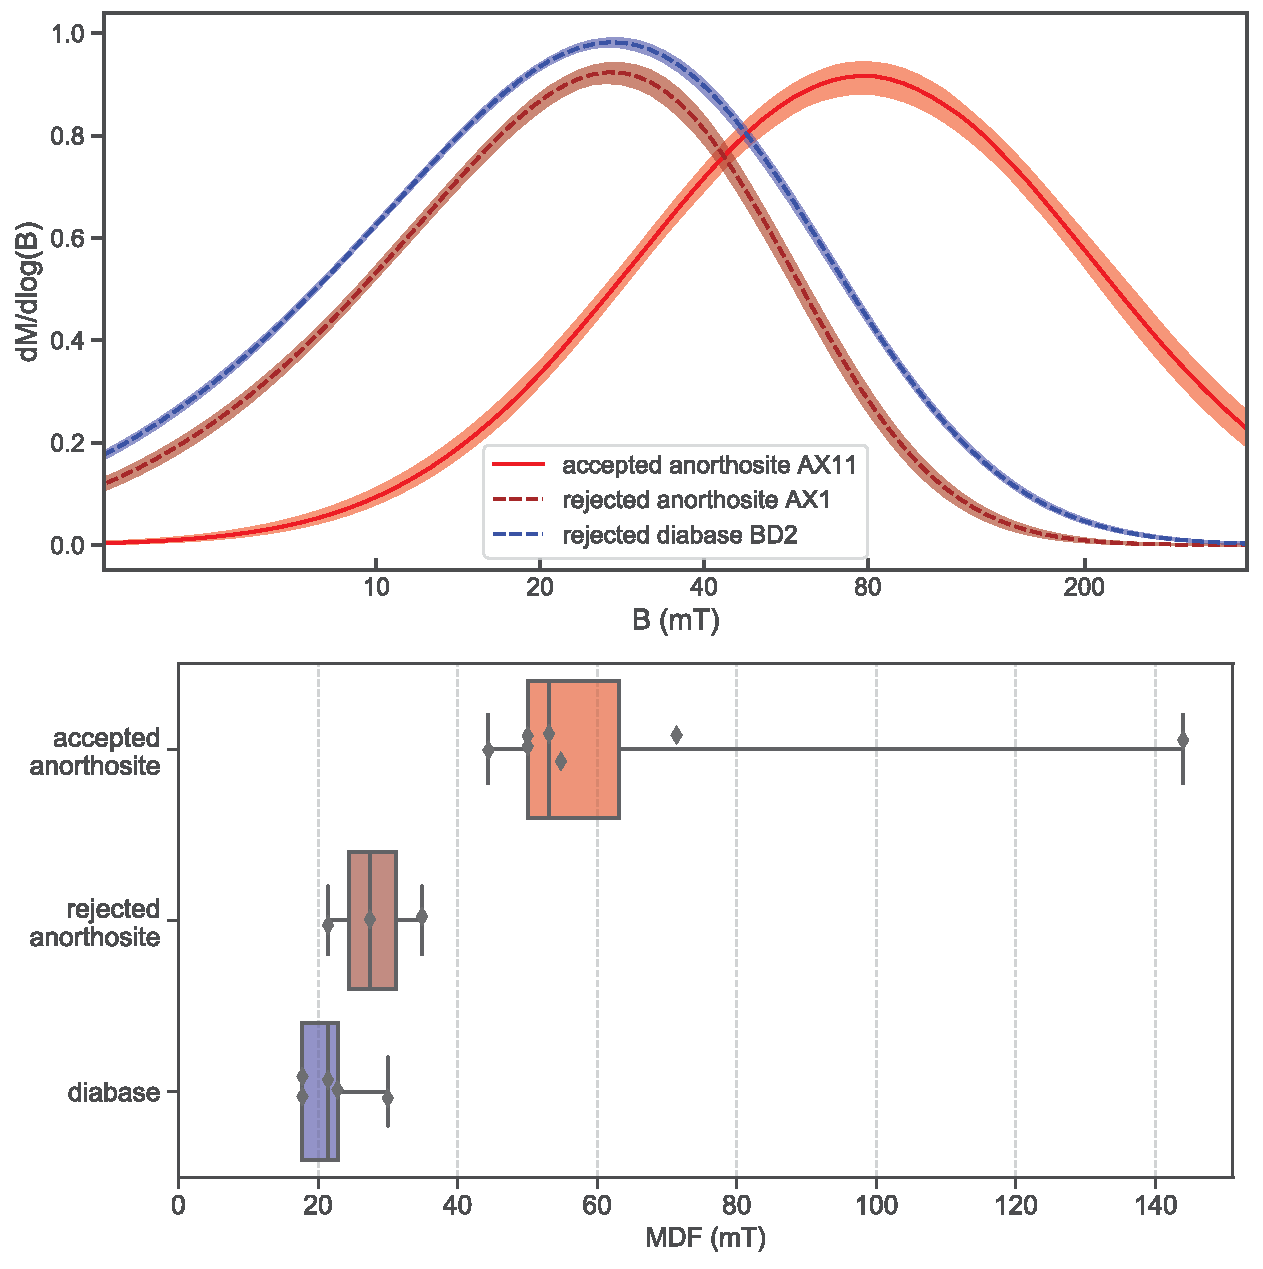
\includegraphics[width=0.58\textwidth]{figure/Zhang2022/coercivity.pdf}
\centering
\caption{\footnotesize{Top: Example coercivity spectra of anorthosite and diabase chips from sites that pass or fail our paleointensity selection criteria. Bottom: Box plots of median destructive field (MDF) values associated with back-field demagnetization for all anorthosite and diabase specimens with single-component coercivity unmixing results. Bars in the boxes show median values and the whiskers show the minimum and the maximum value of the datasets. Both plots show that anorthosite specimens that pass paleointensity selection criteria have higher coercivities consistent with a higher portion of single-domain-like magnetite grains than the other anorthosite specimens and the diabase.}}
\label{fig:coercivity}
\end{figure}

\subsubsection*{Bulk TRM anisotropy}
Significant remanence anisotropy has been documented to exist within certain anorthositic rocks that formed in layered intrusive complexes \citep{Selkin2000a, Feinberg2006a}. Strong remanence anisotropy associated with the igneous foliation developed within anorthosite from the Stillwater Complex has been shown to cause significant overestimation or underestimation of paleointensity values depending on the relative orientations between the fabrics and an applied magnetic field \citep{Selkin2000a}. To assess whether our paleointensity estimates are biased by bulk remanence anisotropy, we calculated the gamma statistic, which is the angular difference between the last pTRM step of paleointensity experiment and the applied field direction. The results show that the anorthosite specimens used in our paleointensity experiment have low gamma values ranging from 0.9\textdegree$\;$ to 11.9\textdegree, with a median value of 4.2\textdegree$\;$(Table S1). Because these anorthosite specimens were oriented at various directions with respect to the outcrops, the angles between the applied lab field direction during paleointensity experiments with respect to any fabrics within the anorthosite specimens are expected to cover a wide range of angles. These gamma values of the anorthosite xenolith bulk specimens are similar to those of the Midcontinent Rift volcanics studied by \citealp{Sprain2018a}. Therefore, the bulk Beaver River anorthosite xenoliths do not have significant remanence anisotropy. Paleodirectional data from our anorthosite xenoliths indicate that they have minimal remanence anisotropy as their site mean directions closely match those of the Beaver River diabase hosts without deviating due to a fabric \citep{Zhang2021b}. These bulk results are consistent with the data from the grain-scale magnetic anisotropy experiments that also show minimal remenance anisotropy (Fig. \ref{fig:Petro_QDM}E, G). 

\subsection*{Considering secular variation and cooling rate}
To best characterize the geomagnetic axial dipole field intensity during a certain time period, a paleointensity dataset should cover a sufficient amount of time such that paleosecular variations of the geomagnetic field are averaged. Thermal modeling results from \citealp{Zhang2021b} indicate that the Beaver River anorthosite xenoliths were heated to tholeiitic magma temperature ($\sim$1100\textdegree C)---lower than the melting temperature of the anorthosite plagioclase (given its composition of 70\% anorthite; \citealp{Morrison1983a, Doyle2016a}) and acquired thermal remanent magnetization during cooling with their diabase host on a time scale of a few thousand years, partially averaging secular variation within single sites. Another consequence of the anorthosite xenoliths having slowly cooled in the interior of thick diabase intrusions is that slow cooling rates can bias paleointensity estimates toward higher values \citep{Halgedahl1980a}. Large differences in cooling rates between acquisition of an NRM in nature versus a TRM in the lab can result in overestimated paleointensities for single domain grains \citep{Dodson1980a, Halgedahl1980a, Nagy2021a}. From the thermal history model of \citep{Zhang2021b}, we can estimate the duration over which the diabase and anorthosite cooled from the Curie temperature of magnetite ($\sim$580\textdegree C) to the time when they blocked in the majority of their characteristic natural remanence magnetization ($\sim$500\textdegree  C; Fig. \ref{fig:IZZI_examples}; \citealp{Zhang2021b}). We find the cooling time to $\sim$500\textdegree C to be $\sim$1.5 kyr, which corresponds to a cooling rate of $\sim1.7\times10^{-9}$ $^\circ$C s$^{-1}$. In contrast, the lab cooling rate is much faster through the same temperature interval with an estimated cooling rate of $\sim1.3\times10^{-1}$ $^\circ$C s$^{-1}$. The significant cooling rate difference leads to a predicted $\sim$33\% overestimate of true ancient field following the model of \citealp{Halgedahl1980a} (Fig. S3). This estimate on cooling rate effect is similar to the value of $\sim$30\% overestimate derived from the model of \citealp{Nagy2021a}. We therefore correct our paleointensity results by a factor of 0.75. Remanence held by vortex state (pseudo-single domain) and multidomain grains is not as biased by cooling rate \citep{Biggin2013a}. The potential for some remanence to be held by these grains, as suggested by slightly zigzagging Arai plots (Fig. \ref{fig:IZZI_examples}), could mean that this factor is an over-correction and true paleointensity values could be slightly higher than those reported here. The cooling rate-corrected specimen paleointensity estimates together with specimen- and site-level means are shown in Fig. \ref{fig:PINT_cooling_corrected}.

Anorthosite xenoliths have paleointensity results that are consistent within small regions, but vary between regions. Anorthosite AX12 (28.65 $\pm$ 4.40 $\mu$T) and AX16 (33.20 $\pm$ 3.82 $\mu$T) in the Silver Bay area were emplaced $\sim$450 meters apart and have indistinguishable paleointensity estimates (Figs. \ref{fig:Chap_PINT_Geologic_map} and \ref{fig:PINT_cooling_corrected}). $\sim$10 km to the north, anorthosite xenoliths AX11 (55.14 $\pm$ 0.05 $\mu$T) and AX13 (57.62 $\pm$ 3.20 $\mu$T) in the Kennedy Creek area were also emplaced closely ($\sim$125 meters apart) and yield similar values to one another, but distinct paleointensity estimates from those of AX12 and AX16 (Figs. \ref{fig:Chap_PINT_Geologic_map} and \ref{fig:PINT_cooling_corrected}). $\sim$30 km further to the north in the Carlton Peak region, AX6 (22.80 $\pm$ 11.41 $\mu$T), AX8 (39.40 $\pm$ 9.14 $\mu$T), and AX10 (35.20 $\pm$ 0.83 $\mu$T) are anorthosite xenoliths within 10 meters of one another and also yield similar paleointensity estimates albeit with relatively large uncertainties (Fig. \ref{fig:PINT_cooling_corrected}). The anorthosites of the three distinct regions captured three different intervals of geomagnetic field intensities during the emplacement and cooling of the Beaver River diabase sills ca. 1092 Ma. To contextualize the high paleointensity values, we plot the regional mean values (Table S3) based on specimen-level paleointensity results together with calculated paleointensity values at 22\textdegree N latitude based on the PADM2M model of the time-varying geomagnetic field over the past 2 million years \citep{Ziegler2011a} in Figure \ref{fig:PINT_cooling_corrected}B. The locality-mean values of these three regions are plotted in Figure \ref{fig:PINT_cooling_corrected}C (and reported in Table S3) where we also present the distribution of means calculated from 3 random values taken from the PADM2M model for a total of 10000 iterations. In addition, we perform the same comparison with the existing paleointensity data for the Cenozoic Era (the last 66 million years) from the PINT database (filtered by Q$_{PI}\geq$3; Fig. S5) given that the observational dataset could record more geomagnetic field excursions or regional high flux patches. The anorthosite xenoliths three region-mean intensity is higher than all values from the resample results of the PADM2M model, and rival the top 3\% values of the resample averages from the Cenozoic data (Fig. S5). This comparison supports that the anorthosite xenoliths record an exceptionally strong geomagnetic field ca. 1092 Ma.

\begin{figure*}[h!]
\noindent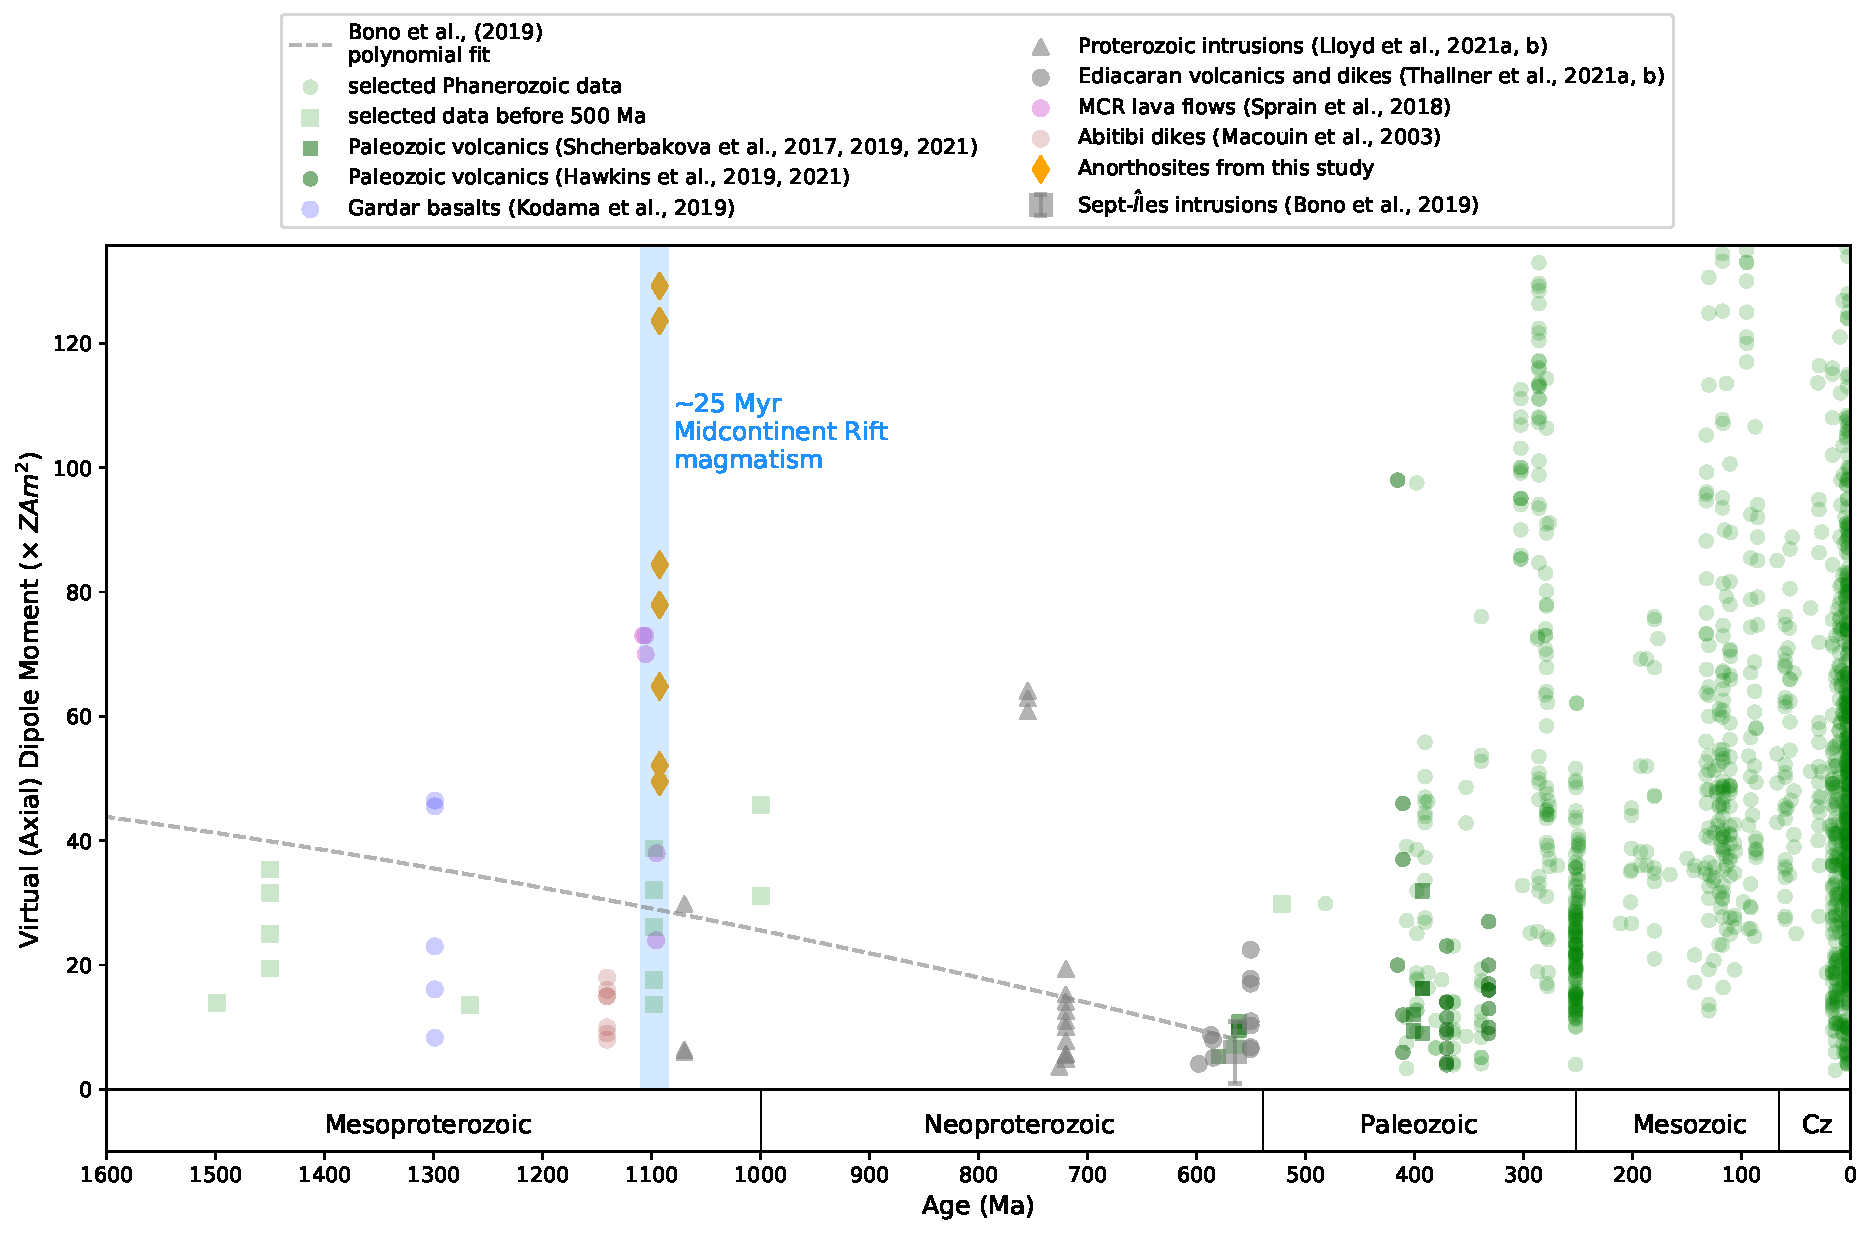
\includegraphics[width=\textwidth]{figure/Zhang2022/PINT_compilation.pdf}
\centering
\caption{\footnotesize{Compilation of calculated virtual (axial) dipole moment values from the PINT database (PINT v8.0.0; \url{http://www.pintdb.org/}; \citealp{Bono2022a}), including all Phanerozoic VDM and VADM records with Q$_{PI}$ values $>$3 and additional Neoproterozoic data from refs. \citealp{Lloyd2021a, Lloyd2021b, Thallner2021a, Thallner2021b}. Paleointensity estimates from refs. \citealp{Pesonen1983a} and \citealp{Kulakov2013a} are not included in the compilation due to the specimen-level double-slope behavior as discussed in the text. Overall, the anorthosite xenoliths from this study record a high Mesoproterozoic field exceeding the value projected by the second order polynomial curve from \citealp{Bono2019a} which is based on an interpretation of there being a monotonic decay of the geodynamo through the Proterozoic. The highest site-mean virtual dipole moment of the anorthosites would rank in the top 2$\%$ of those in the database for the Cenozoic Era (the last 66 million years) when there was unequivocally a crystallizing inner core. The y-axis maximum is set at the 99th percentile of the compiled Cenozoic paleointensity data.}}
\label{fig:PINT_compilation}
\end{figure*}

\section{Discussion}

The crystallization of the solid inner core is an important event in the long-term evolution of Earth's core and in sustaining the geodynamo \citep{Buffett2000a}. The age of the inner core in thermal evolution models relies on estimates for the thermal conductivity of iron alloys at the temperatures and pressures of the core \citep{Ohta2021a}. Prior to studies of the last 10 years, an accepted value of $\sim$30 W m$^{-1}$ K$^{-1}$ for this thermal conductivity constrained the timing of inner core nucleation to be during the first half of Earth's history \citep{Stacey2007a, Konopkova2016a}. Subsequently, experimental data and \textit{ab intio} simulations were interpreted to imply higher thermal conductivity values \citep{Pozzo2012a, Ohta2016a} which in turn implied a younger age for the inner core ($<$700 Ma; \citealp{Labrosse2015a}). However, other experimental studies continue to indicate lower thermal conductivity values consistent with prior estimates \citep{Konopkova2016a, Hsieh2020a} with no consensus yet emerging \citep{Williams2018a, Ohta2021a}. These experiments are challenging to conduct and interpret given complexities such as constraining the sample thickness under high pressure and temperature conditions, the validity of applying the Wiedemann-Franz law to extrapolate thermal conductivity values based on electrical resistivity measurements \citep{Ohta2016a}, and propagating uncertainties from free parameters used in finite element modeling of direct thermal conduction experiments \citep{Konopkova2016a}. Further experiments and theory are needed to explain these contrasting results which at present leave open very different trajectories for Earth's thermal evolution. As a result, the age of the inner core is relatively unconstrained from a theoretical perspective. 

The other data type that can provide insight into the long-term history of the core's thermal regime and geodynamo is paleomagnetic data---both paleodirectional data that indicate the presence of a geomagnetic field and paleointensity data that constrain the field's strength. Inner core nucleation would have increased the power to the geodynamo which has the potential to manifest as an increase in Earth's surface field \citep{Davies2021a}. An approach combining dynamo simulations and theoretical scaling relationships has predicted that progressive decay of the field's dipole moment would be followed by a rapid increase in geomagnetic field intensity soon after the onset of inner core nucleation such that a minimum in dipole moment would occur just before inner core nucleation \citep{Davies2021a}. Other scenarios are possible, however, such as the model-based prediction that while power increases associated with inner core nucleation strengthen Earth's internal magnetic field, that the dynamo becomes more deeply seated in the core diminishes the increase in magnetic field strength at Earth's surface \citep{Aubert2009a, Landeau2017a}. Such a scenario where the dynamo shifts to a greater depth associated with inner core nucleation led \citealp{Aubert2009a} to conclude that the increase in power to the dynamo would be difficult to detect with paleointensity data. Ultimately, further observational paleomagnetic records are key as they hold the potential for testing different model predictions and identifying transitions in ancient field strength \citep{Biggin2015a, Bono2019a}.

It has been proposed that Proterozoic paleointensity data are consistent with a progressive monotonic decay leading to a minimum ca. 565 Ma in the Ediacaran Period (Fig. \ref{fig:PINT_compilation}; \citealp{Bono2019a}). This interpretation was motivated by paleointensity estimates developed from the ca. 565 Ma Sept-$\hat{I}$les layered mafic intrusive complex of $\sim$7 ZAm$^2$ that are among the lowest values in the paleointensity database (Fig. \ref{fig:PINT_compilation}; \citealp{Bono2019a}). A decay in the lead-up to this time was argued to be consistent with an absence of an inner core and a dynamo to which progressively less power was available through secular cooling \citep{Bono2019a, Davies2021a}. This timing of inner core formation would favor a high core thermal conductivity \cite[e.g.][]{Ohta2016a}. Paleomagnetic directional excursions \citep{Halls2015a}, other weak paleointensity estimates \citep{Thallner2021b}, and frequent polarity reversals \citep{Kodama2021a} in rocks of similar age are interpreted to be consistent with numerical simulations \citep{Driscoll2016a} associated with a weak dipole field. 

The high paleointensity estimates from the 1.1 billion-year-old Midcontinent Rift rocks challenge the hypothesized monotonic decay of the geomagnetic field strength throughout the Proterozoic Era (Fig. \ref{fig:PINT_compilation}). The well-preserved ca. 1092 Ma anorthosite xenoliths of the Beaver River diabase record a strong geomagnetic field in the late Mesoproterozoic that exceeds the modern-day field strength for which crystallization of the inner core is a power source (Figs. \ref{fig:PINT_cooling_corrected} and \ref{fig:PINT_compilation}). Together with previous records obtained from the ca. 1106 Ma Osler Volcanics of the Midcontinent Rift \citep{Sprain2018a}, these data indicate that appreciable power to Earth's dynamo persisted through at least 14 Myr during the late Mesoproterozoic to maintain a strong surface field (Fig. \ref{fig:PINT_compilation}). In addition to these high geomagnetic fields recorded by Midcontinent Rift rocks, the ca. 755 Ma Mundine Well dikes \citep{Lloyd2021b} also require a stronger geomagnetic field in the Neoproterozoic than would be predicted by a progressive Proterozoic decline. Taken together, these results call into question whether the progressively decaying polynomial fit implemented by \citep{Bono2019a} is an accurate representation for the evolution of the Proterozoic geomagnetic field (Fig. \ref{fig:PINT_compilation}). 

The hypothesis that a weak Ediacaran geomagnetic field is a telltale sign of the lack of an inner core with core nucleation following shortly thereafter may predict that it is the most significant weak to strong field transition in the paleointensity record. However, Fig. \ref{fig:PINT_compilation} shows that transitions from low to high field intensities occurred before, during, and after the Ediacaran Period. In the Ediacaran record developed to date, there is a two-fold increase in Earth's virtual dipole moment when comparing estimates from the ca. 565 Ma Sept-$\hat{I}$les intrusions \citep{Bono2019a} to those from ca. 550 Ma volcanics of the Skinner Cove Formation (Fig. \ref{fig:PINT_compilation}; \citealp{Thallner2021a}). In the late Mesoproterozoic, there is at least a six-fold increase within a period of $\sim$35 Myr from a low average virtual dipole moment of $\sim$13 ZAm$^2$ recorded by the ca. 1140 Ma Abitibi dikes which yielded straight Arai plots \citep{Macouin2003a}, to a high moment of $\sim$70 ZAm$^2$ recorded by the ca. 1106 Ma Osler Volcanics, with even stronger values from ca. 1092 Ma by Beaver River anorthosite xenoliths that record virtual dipole moments up to $\sim$129 ZAm$^2$. While the ca. 1140 Abitibi dikes' paleointensity estimates are not as low as those of the ca. 565 Ma Sept-$\hat{I}$les intrusions, this virtual dipole moment increase in the Mesoproterozoic from the ca. 1140 Ma data to the ca. 1100 Ma data is the largest yet documented in the Precambrian on a 10s of millions of years timescale (Fig. \ref{fig:PINT_compilation}). The tempo and scale of this field intensity transition could match with model-based predictions associated with the onset of inner core nucleation \citep{Davies2021a}. This ca. 1.1 Ga timing would be broadly consistent with the ca. 1.3 Ga onset proposed by \citealp{Biggin2015a} albeit later given the exclusion of previous overestimated paleointensity values from the ca. 1.3 Ga Gardar basalts that are superseded by data in \citealp{Kodama2019a}. However, a model prediction of sustained strong field values following inner core nucleation is challenged by data from the ca. 1070 Ma Bangemall Sills which include a sill with a low virtual dipole moment of $\sim$6.4 ZAm$^2$ (Fig. \ref{fig:PINT_compilation};  \citealp{Lloyd2021b}). Following the Ediacaran, there are also low paleointensity estimates from Devonian rocks such as the ca. 370 Ma dikes and lavas of the Siberian Viluy Traps that give virtual dipole moment estimates of 4.3 to 14.9 ZAm$^2$ (Fig. \ref{fig:PINT_compilation}; \citealp{Hawkins2019a}). These low values as well as data from the ca. 414 Ma Strathmore lava flows \citep{Hawkins2021a}, the ca. 410-380 Ma lava flows of Siberia and the Kola Peninsula \citep{Shcherbakova2017a}, the ca. 408–393 Ma Buribay volcanics \citep{Shcherbakova2021a} and the ca. 332 Ma Kinghorn volcanics \citep{Hawkins2021a} have led to the proposal of this interval being the ``Mid-Paleozoic Dipole Low'' \citep{Hawkins2021a}. This ``Mid-Paleozoic Dipole Low'' is followed by high paleointensity values such that there is a six-fold increase from virtual dipole moments of $\sim$16 ZAm$^2$ ca. 332 Ma to $\sim$99 ZAm$^2$ ca. 308 Ma in the late Carboniferous (Fig. \ref{fig:PINT_compilation}; \citealp{Hawkins2021a}). 

Given that the multiple records of a weak field in the Proterozoic and Paleozoic cannot all be the minimum prior to the singular event of the onset of inner core nucleation, what processes could lead to a weak dipole at Earth's surface even in the presence of a crystallizing inner core? Numerical models have shown that the dipole moment is sensitive to both the magnitude and spatial pattern of heat flow across the core-mantle boundary when there are strong available power sources to the geodynamo \citep{Olson2007a, Olson2010a}. In such models, relatively low total heat flux across the core-mantle boundary can prevent the axial dipole from reversing whereas a high heat flux through the boundary can result in an increase in reversal frequency and decrease in dipole intensity. The ``Mid-Paleozoic Dipole Low'' has been hypothesized to be the result of such elevated core-mantle boundary heat flux conditions at a time when there was also available power from a crystallizing inner core \citep{Hawkins2019a}, thereby also explaining the observed low paleointensities which include values as weak as those of the ca. 565 Ma Sept-$\hat{I}$les intrusions (Fig. \ref{fig:PINT_compilation}; \citealp{Bono2019a}). Mantle convection can modulate core mantle boundary heat flow through changes in the structure of the deep mantle associated with upwelling plumes \citep{Larson1991a, Courtillot2007a} and subducted slabs \citep{Tan2002b, Biggin2012a, Hounslow2018a}. Strong evidence for differential plate tectonic motion extends back to ca. 2.2 Ga in the Paleoproterozoic \citep{Mitchell2014a, Swanson-Hysell2021b} and potentially back to ca. 3.2 Ga in the Archean \citep{Brenner2020a}. Plate tectonic modulations of core mantle boundary heat flow are therefore expected throughout the Proterozoic. Such changes may explain large variability in Proterozoic paleointensity values similar to those seen in the Phanerozoic \citep{Lloyd2021a} and may challenge our ability to detect the increase in surface geomagnetic field strength predicted to have happened at the onset of inner core crystallization. 

Overall, the high-fidelity paleointensity recorders of the Beaver River anorthosite xenoliths in the well-preserved Midcontinent Rift record strong field strengths 1.1 billion years ago. The highest site-level value of the virtual dipole moment would rank in the top 2$\%$ of those in the database for the Cenozoic Era when there was unequivocally a crystallizing inner core. These high surface field strengths necessitate that appreciable power was provided to the late Mesoproterozoic geodynamo. 

\section{Methods}
\subsection*{Sample collection and paleomagnetic directions}

We collected paleomagnetic cores that are 2.5 cm in diameter along the southern and eastern Beaver Bay Complex with a particular focus on acquiring paired sites of anorthosite xenoliths and their local diabase hosts during summer field seasons in 2019 and 2020. Sample cores were collected using a hand-held gasoline-powered drill and were oriented using a magnetic compass as well as a sun compass when possible. Sun compass orientations were preferentially used for determining the sample azimuth. Sister specimens underwent step-wise alternating field (AF) or thermal demagnetization at the UC Berkeley Paleomagnetism Lab to isolate paleomagnetic directions (data presented in \citealp{Zhang2021b}). Based on the anorthosite thermal demagnetization results, we selected sites whose unblocking temperature ranges are narrow and near 580\textdegree C for paleointensity experiments. Beaver River diabase sites with minimal secondary remanence were also selected for paleointensity experiments. 

\subsection*{Paleointensity experiment}
A total of 86 specimens from 14 anorthosite xenoliths and a total of 69 specimens from 7 diabase sites underwent paleointensity experiments that followed the step-wise double-heating Thellier method \citep{Thellier1959a} using the IZZI protocol \citep{Yu2004a} with heating steps up to 585 \textdegree C. Partial thermal remanent magnetization (pTRM) checks were performed systematically throughout the experiment to test whether there was significant mineralogical alteration due to heating and were assessed using the SCAT parameter of  \citealp{Shaar2013a}. On top of the IZZI-Thellier experiment protocol, we also performed a comparative study where we added an extra step of 20 mT alternating field (AF) cleaning on some of the specimens after each in-field step. The purpose was to study whether the AF cleaning could help improve experiment success rate by removing the remanence component carried by materials such as multi-domain (MD) grains that contribute to non-ideal paleointensity behaviors. The results were similar when this step was applied without an observed change in experimental success rate. All remanence measurements were made on a 2G Enterprises DC-SQUID superconducting rock magnetometer equipped with an automated sample changer system at the UC Berkeley Paleomagnetism laboratory. The magnetometer is housed inside a three-layer magnetostatic shield that maintains background fields of less than 500 nT. Heating steps were performed using an ASC TD-48SC thermal demagnetizer with a controlled field coil that allows for a magnetic field to be generated in the oven in conjunction with a DC power supply. The thermal demagnetizer was degaussed with an alternating field in the axial orientation following each in-field step such that residual fields within the oven were $<$10 nT during zero-field steps. Samples were placed in the same location within the thermal demagnetizer for each heating step and were maintained in the same orientation with regard to the applied field. During each heating step, the oven remained at peak temperatures for 20 min to make sure each specimen reached the target temperature. An applied laboratory field of 30 $\mu$T was used for all in-field steps. All heating steps were performed in air. The temperature increments for the experiments were chosen to isolate magnetizations held by (titano)magnetite informed by the previous demagnetization data, with smaller increments performed close to $\sim$580\textdegree C. 

\subsection*{Paleointensity result selection}
The following criteria were used as quality filters on the paleointensity results: (1) a maximum angular deviation (MAD;  \citealp{Kirschvink1980a}) of $<$10\textdegree; (2) scatter parameter ($\beta$;  \citealp{Coe1978a}) values of $<$15$\%$; (3) a deviation angle (DANG;  \citealp{Tauxe2004a}) of $<$5\textdegree; (4) fraction of remanence fitted for paleointensity estimate (FRAC;  \citep{Shaar2013a}) $>$0.6; (5) scatter statistic (SCAT;  \citealp{Shaar2013a}) = TRUE; (6) a maximum magnetic moment difference between adjacent zero-field steps (GAP-Max;  \citealp{Shaar2013a}) $<$ 0.25; (7) number of pTRM checks $>$ 2; (8) and number of measurements used for paleointensity determination $\geq$ 4. MAD measures the scatter about the best-fit line through the natural remanent magnetization (NRM) steps in the selected interval for which the intensity is defined. DANG, the deviation angle, is the angle between the best-fit direction that is free floating and the direction between the center of mass of the data and the origin of the vector component diagram \citep{Tauxe2004a}. Both MAD and DANG assess the directional variation of the NRM, with MAD measuring the scatter in the NRM directions and DANG assessing whether the component is trending toward the origin of the Zijderveld plot. $\beta$ is the ``scatter" parameter of  \citep{Coe1978a} and is the ratio of the standard error of the slope of the best-fit line of the selected NRM and pTRM points on an NRM/TRM plot to the absolute value of the slope. FRAC is the fraction of the NRM that is used in the best-fit line \citep{Shaar2013a}. The FRAC value was chosen to preferentially select samples with dominantly single-slope NRM/TRM plots. GAP-Max is the maximum gap between two points on the NRM/TRM plot determined by vector arithmetic. SCAT is a Boolean operator which uses the error on the best-fit slope of the selected data on the NRM/TRM plot to determine if the data are overly scattered. The parameter is used to assess pTRM checks in addition to assessing the degree to which IZZI steps are zigzagged. $\beta$, FRAC, GAP-Max and SCAT are all statistics to assess the behavior of NRM/TRM plots. See the Standard Paleointensity Definitions (\citealp{Paterson2014a}; \url{https://earthref.org/PmagPy/SPD/home.html}) for more details. Data analysis was conducted using Thellier GUI \citep{Shaar2013a} within the PmagPy software package \citep{Tauxe2016a}.

\subsection*{Rock magnetic experiments}

We conducted rock magnetic experiments to characterize the magnetic mineralogy and gain insights into the paleointensity results of the anorthosite and diabase. Back-field curves were measured at room temperature using a Micromag Princeton Measurements vibrating sample magnetometer (VSM) and a Lake Shore 8600 series VSM at the Institute for Rock Magnetism. Specimen median destructive fields (MDF) were calculated based on the back-field experiments. The calculated coercivity spectra were subsequently decomposed into one or more components using skew-normal distributions following the method of  \citealp{Maxbauer2016a} examples of which are shown in Fig. \ref{fig:coercivity}. We also used a magnetic property measurement system (MPMS) at the Institute for Rock Magnetism to aid the identification of magnetic minerals. In the field-cooled (FC) experiments, specimen magnetizations were measured upon warming following the specimen having cooled in an applied field of 2.5 T from 300 to 10 K. In the zero-field-cooled (ZFC) experiment, a low-temperature saturation isothermal remanence (LTSIRM) of 2.5 T was applied at 10 K after the specimen cooled in a (near-)zero field. In the room-temperature saturation isothermal remanence (RTSIRM) experiment, the sample was pulsed with a 2.5 T field at room temperature ($\sim$300 K) and then cooled to 10 K and warmed back to room temperature in a (near-)zero field. The magnetic moment transitions at critical temperatures shown through MPMS experiments were used to identify magnetic minerals such as magnetite within specimens \citep{Feinberg2015a}. 

To further identify the magnetic carriers within the Beaver River anorthosite xenoliths and compare them with the anorthosites of the Duluth Complex Anorthositic Series rocks, we used the quantum diamond microscope (QDM) at the UC Berkeley Paleomagnetism laboratory to image a thin section of sample MS99033 from anorthosite xenolith AX16 (which yielded a $^{206}$Pb/$^{238}$U zircon date of 1091.83 $\pm$ 0.21 Ma;  \citealp{Zhang2021b}), and a thin section of a Duluth Complex anorthosite (Fig. \ref{fig:Petro_QDM}). We use the QDM to image the magnetic field over the polished thin section surfaces with a sample-sensor distance of $\sim$5 $\mu$m in projective magnetic microscopy (PMM) mode with a spatial resolution of 4.7 $\mu$m per pixel and an instantaneous 0.9 mT bias field that is canceled during the course of measurement \citep{Glenn2017a}.

\section{Acknowledgements}

Project research was supported by NSF CAREER grant EAR-1847277 to N.L.S.-H., an Institute on Lake Superior Geology Student Research Fund grant to Y.Z., and an Institute for Rock Magnetism Visiting Student Fellowship to Y.Z. The Institute for Rock Magnetism is supported by the Instrumentation and Facilities program of the NSF Earth Science Division. Permits for fieldwork and sampling from the Minnesota Department of Natural Resources are gratefully acknowledged. We thank James Pierce and Blake Hodgin for their assistance in the field. We thank Jim Miller for providing us with the Duluth Complex anorthosite thin section. We thank Dario Bilardello, Peat Solheid, Mike Jackson, Josh Feinberg, and Bruce Moskowitz for their tremendous help with instrument operation, data interpretations, and research guidance at the IRM. Conversations with Bruce Buffett and Zachary Geballe informed our perspectives on the geodynamic and mineral physics literature. We thank Jon Hagstrum at USGS and two anonymous reviewers for their helpful comments on the manuscript.
